\pagebreak
\subsection{Convergencia de la norma}

En este experimento vamos a anlizar como varia la convergencia de la norma segun el valor de $c$. Para hacer esto vamos a emplear tres instancias SNAP, estas son:

\begin{itemize}
	\item Berkeley-Stanford (Nodos: 685230 Ejes: 7600595)
	\item Notre Dame (Nodos: 325729 Ejes: 1497134)
	\item Stanford (Nodos: 281903 Ejes: 2312497)
\end{itemize}
	
\subsubsection{Tiempos de convergencia}

Para cada una de las instancias el tiempo de convergencia segun $c$ fue el siguiente:

\begin{figure}[h]
\centering
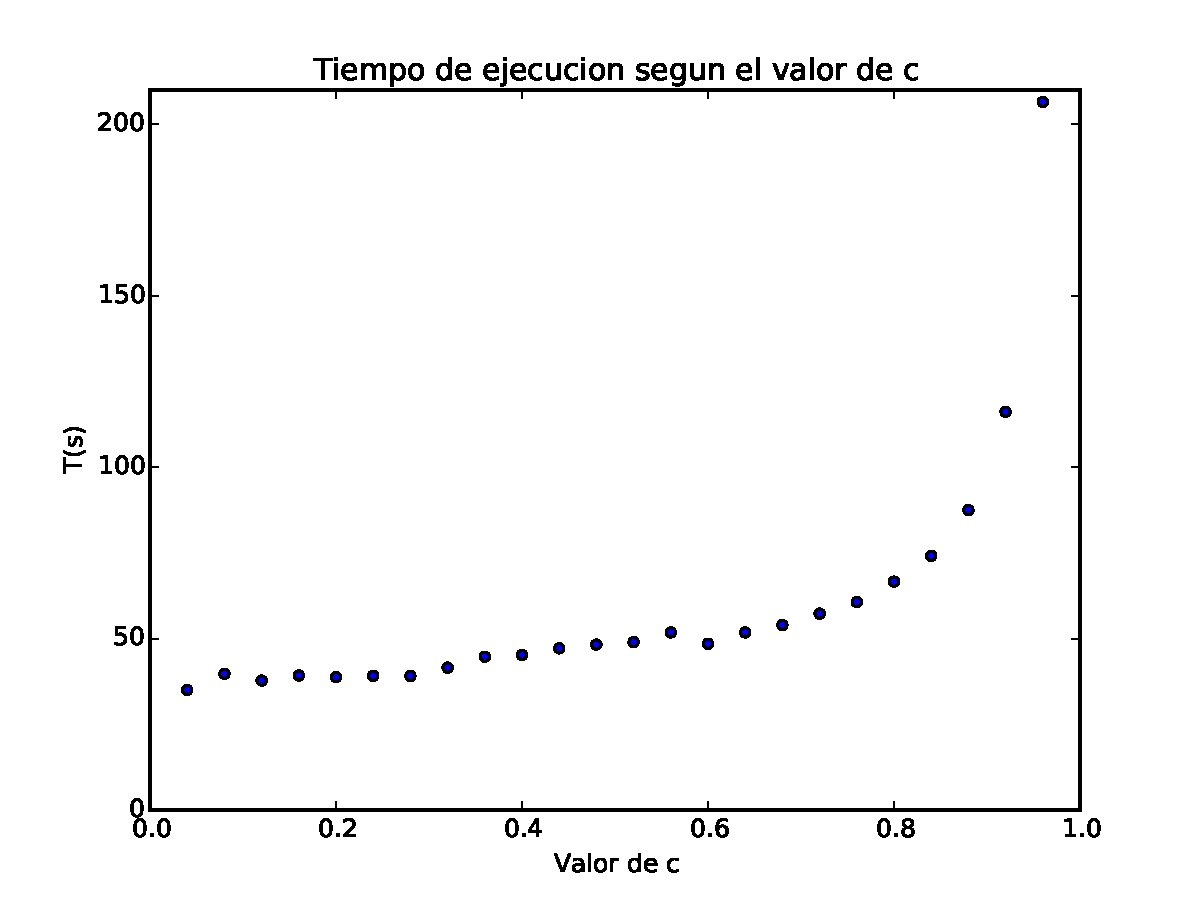
\includegraphics[scale=0.5]{images/web-BerkStan.pdf}
\caption{Instancia Berkeley-Stanford}
\label{timePageRank}
\end{figure}

\begin{figure}[h]
\centering
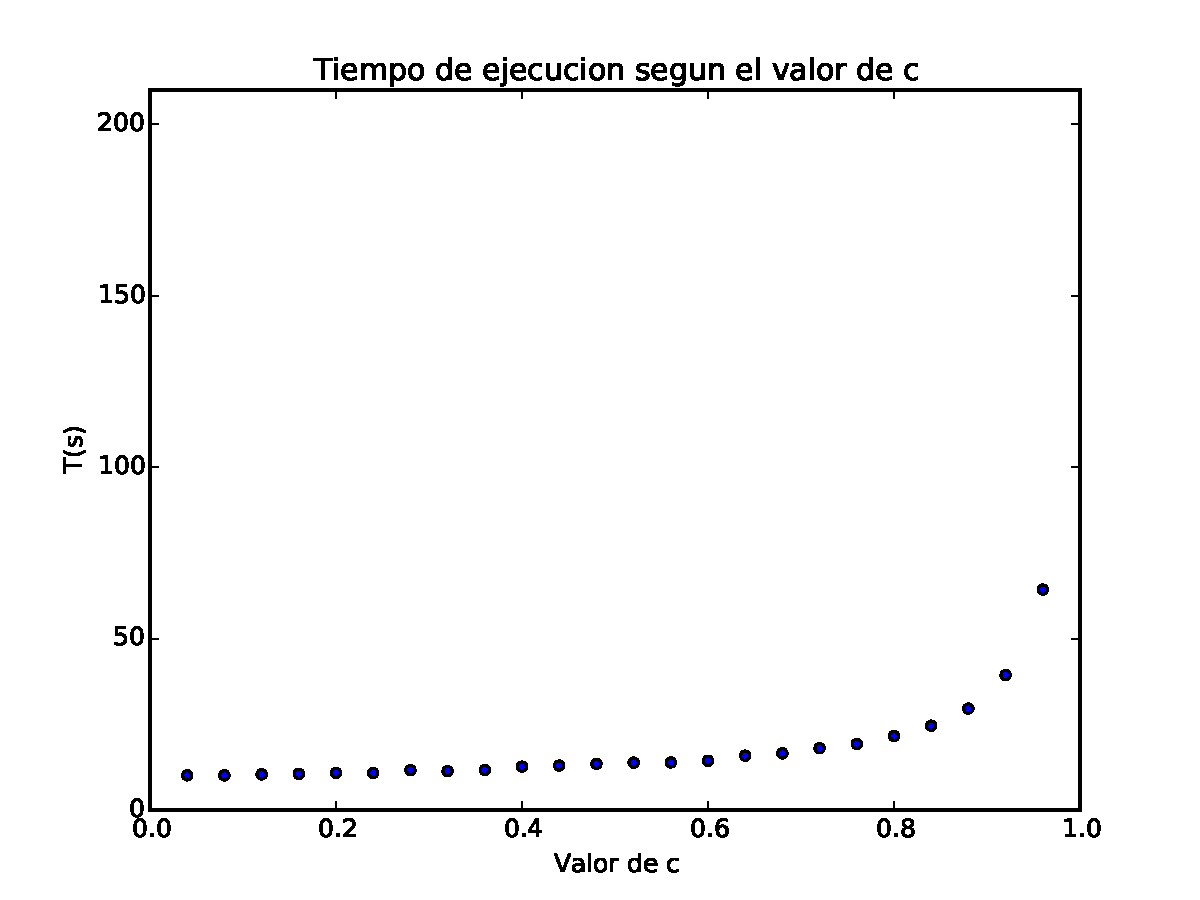
\includegraphics[scale=0.5]{images/web-NotreDame.pdf}
\caption{Instancia Notre Dame}
\label{timePageRank}
\end{figure}

\newpage

\begin{figure}[h]
\centering
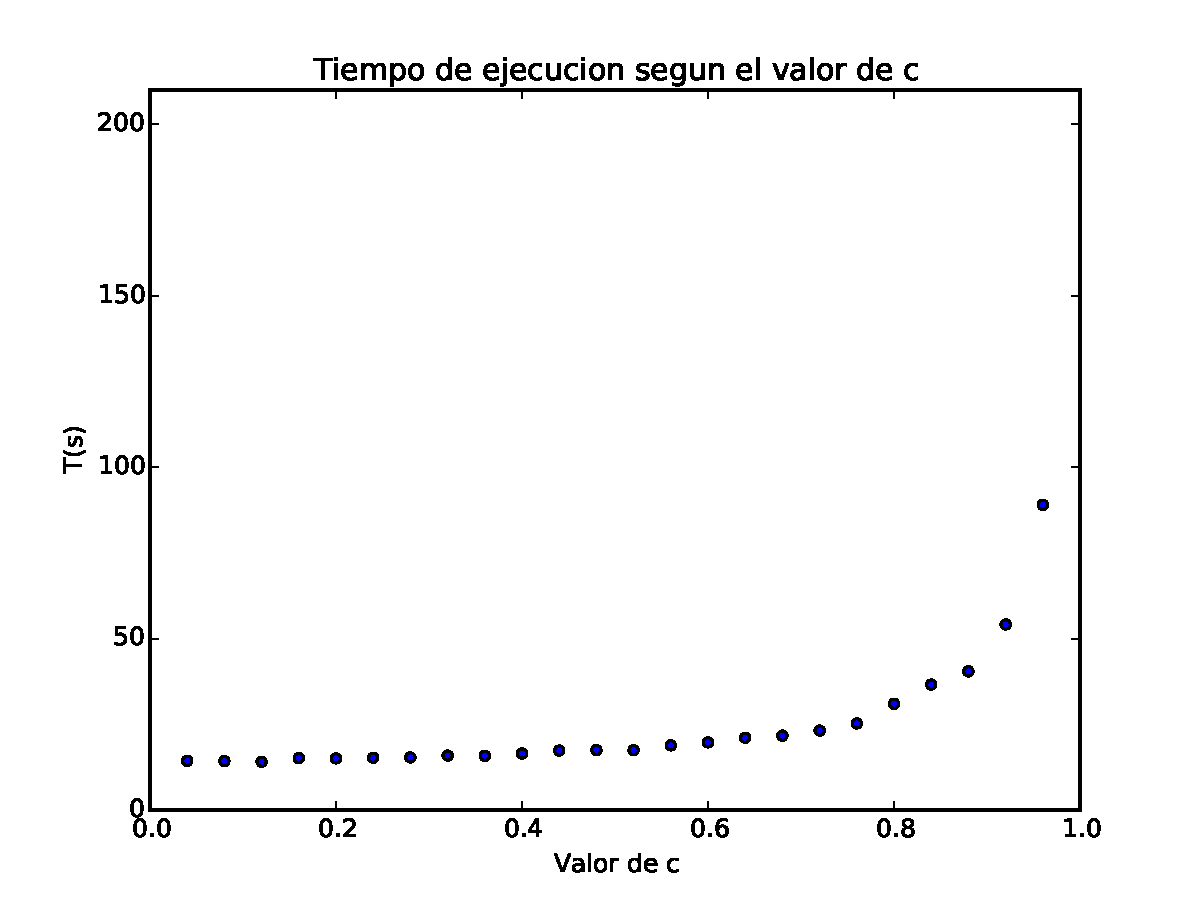
\includegraphics[scale=0.5]{images/web-Stanford.pdf}
\caption{Instancia Stanford}
\label{timePageRank}
\end{figure}

Como podemos apreciar, si bien la instancia Berkeley-Stanford fue la que mas tardo en converger, para valores de $c$ hasta 0.9 la diferencia en tiempo no fue grande. Este es un resultado importante que se condice con el paper de Page y Brin, el algoritmo escala de manera muy eficiente a los diferentes tamaños de entrada, ya que por ejemplo Berkley-Stanford tiene mas del doble de nodos y seis veces mas ejes que Notre Dame, sin embargo la difirencia en tiempo entre las instancias es pequeña. El aumento en tiempo de convergencia tambien se coincide con la idea del navegante aleatorio, la norma va a tardar menos en converger con valores bajos de $c$ ya que el usuario recorreria la web de manera mucho mas veloz (y erratica) que con valores altos.

\subsubsection{Evolucion de la norma}

Como vimos antes, los casos con valor de $c$ entre 0.8 y 0.96 son los que mas tardan en converger, con lo cual tenemos suficientes datos como para estudiar la convergencia de la norma. Vamos a ver los casos para $c$ igual a 0.8, 0.84, 0.88 para la instancia Berkeley-Stanford:

\begin{figure}[h]
\centering
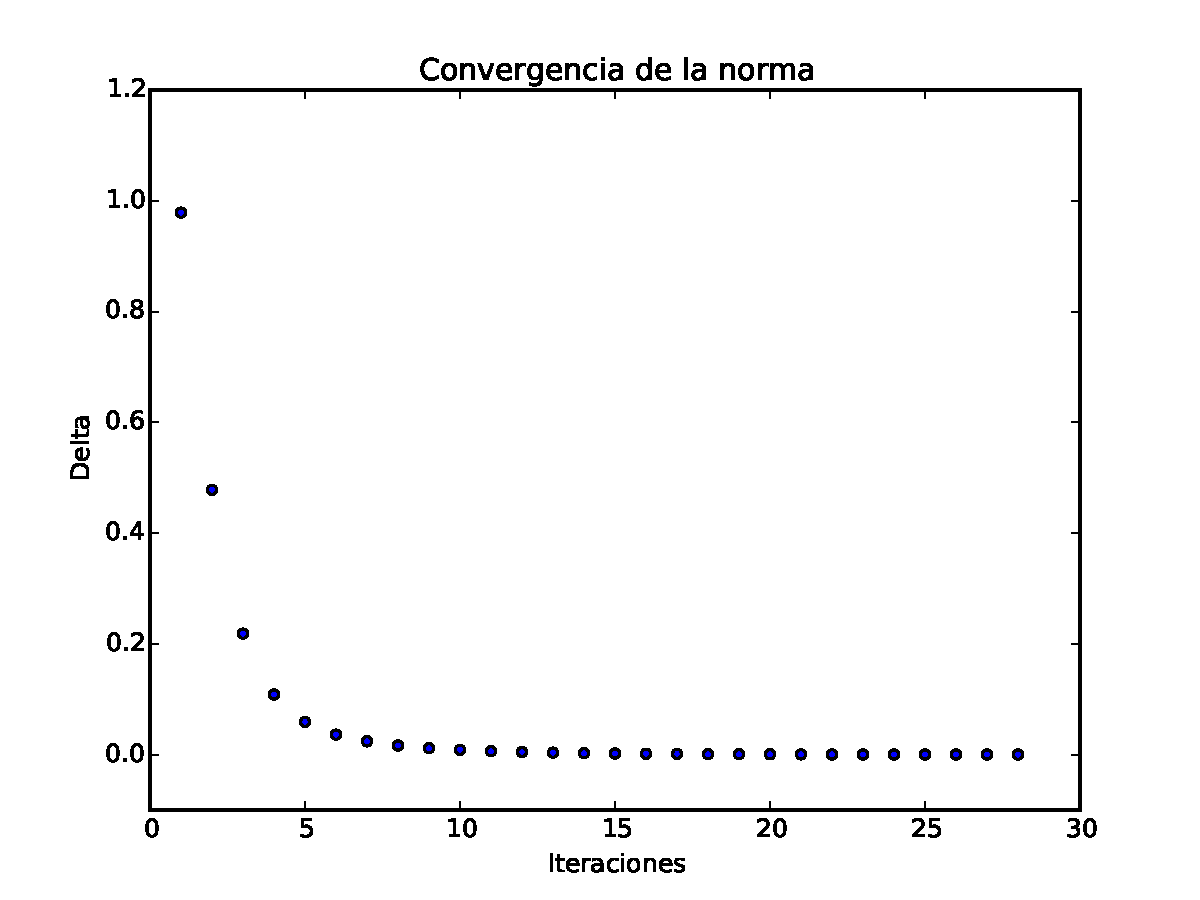
\includegraphics[scale=0.4]{images/normas/web-BerkStan_20.pdf}
\caption{Instancia Berkeley-Stanford ($c$ = 0.8)}
\label{timePageRank}
\end{figure}

\newpage

\begin{figure}[h]
\centering
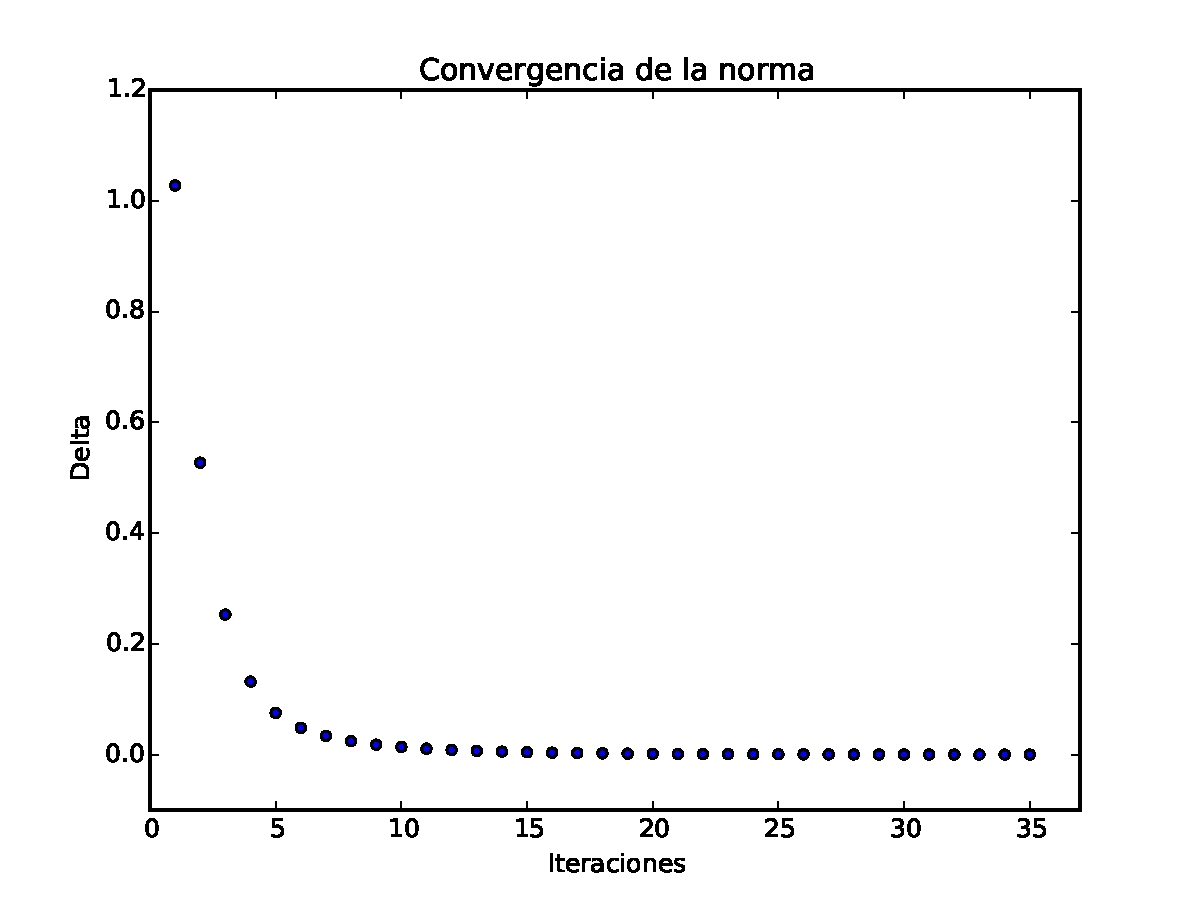
\includegraphics[scale=0.4]{images/normas/web-BerkStan_21.pdf}
\caption{Instancia Berkeley-Stanford ($c$ = 0.84)}
\label{timePageRank}
\end{figure}

\begin{figure}[h]
\centering
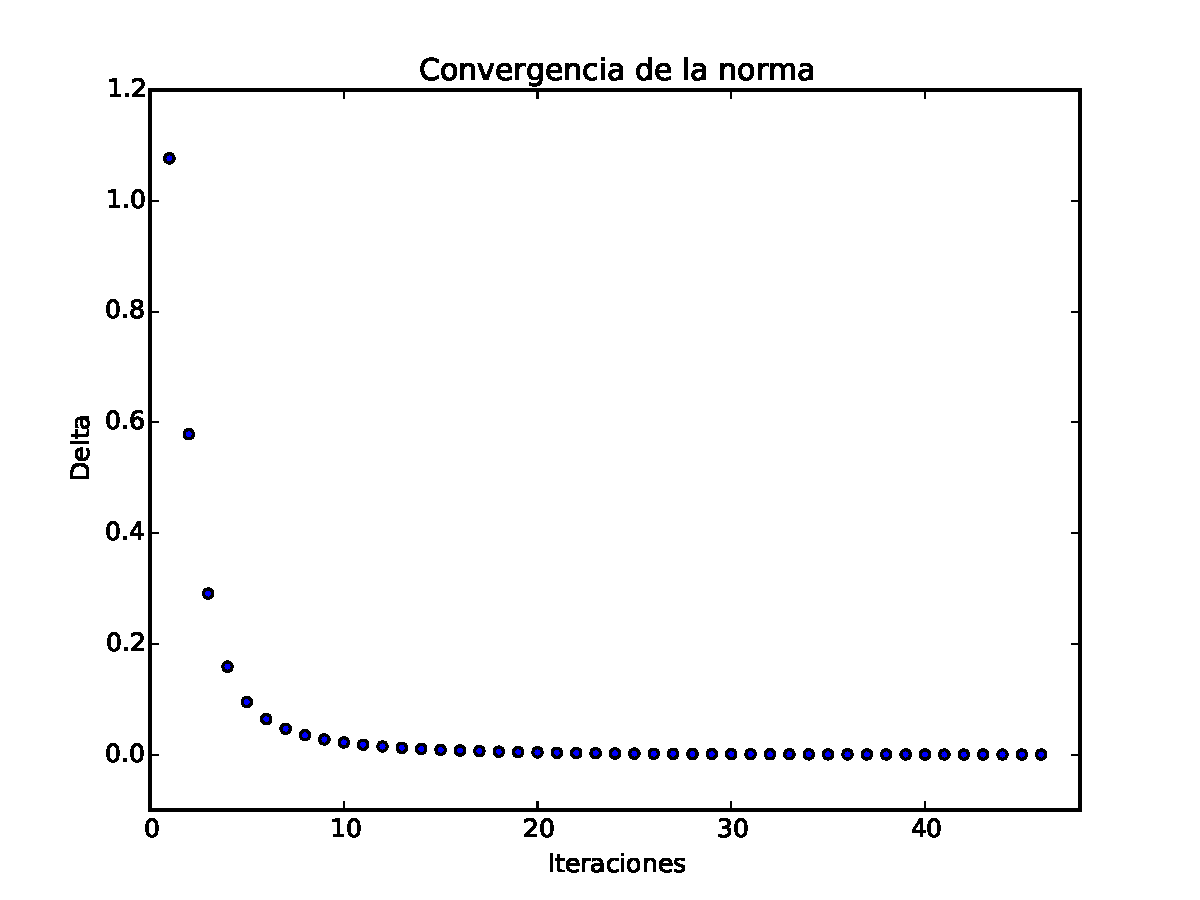
\includegraphics[scale=0.4]{images/normas/web-BerkStan_22.pdf}
\caption{Instancia Berkeley-Stanford ($c$ = 0.88)}
\label{timePageRank}
\end{figure}

Como se puede ver, a medida que el valor de $c$ aumenta, la cantidad de iteraciones para llegar a la convergencia se incrementa en mas de un 10\% en cada aumento, si bien en este caso pequeño la diferencia puede ser despreciable, esto puede traer implicaciones importantes para casos mas grandes. Desde el punto de vista de convergencia, a menor valor de $c$, mas rapida es la convergencia de la norma, sin embargo tambien queda analizar como impacta en el ranking los diferentes valores de $c$, esto se vera en las proxima secciones.